\section{当前面对的困境:宏观压力、增长降速}

过去一年 Atlassian 增长动力在许多方面都受到了挑战,当前面临的困境既有外部高通胀、高利率、强竞争等因素影响,也有企业内部战略选择、产品能力有关。

\textbf{宏观逆风抑制免费用户转化率与现有用户付费意愿}。尽管云计算成为了企业必要支出,但在当前通货膨胀、能源价格上涨、美元加息影响持续,企业正减少支出以应对市场的不确定性,短期内企业在云计算上的投入相对保守,影响飞轮的转化。
\begin{figure}[H]
    \caption{宏观逆风显现,全球云计算增速放缓}
    \begin{center}
        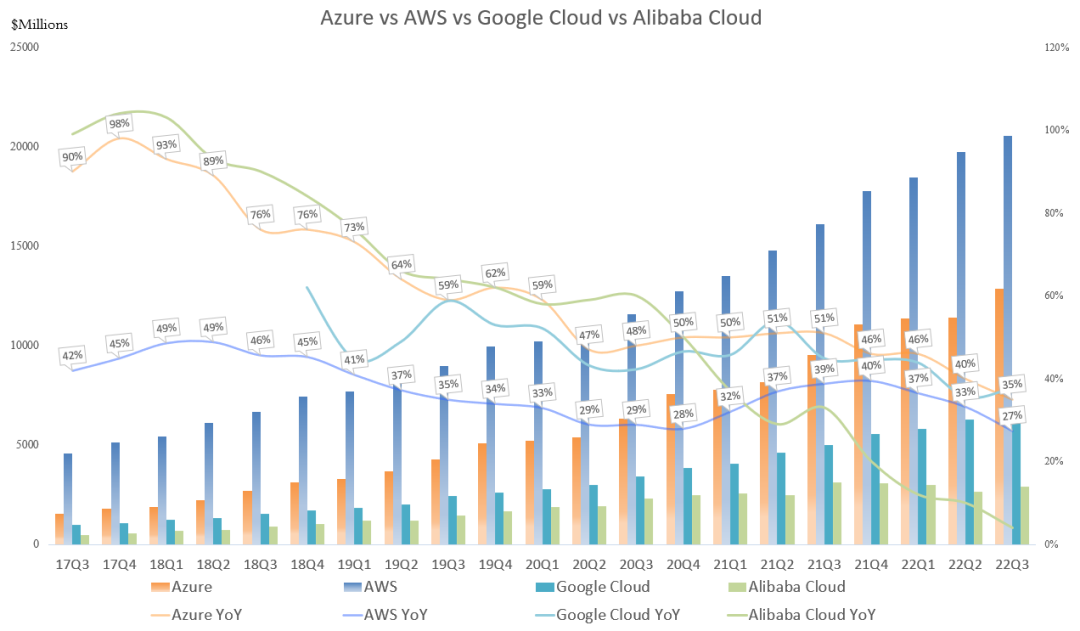
\includegraphics[width=\linewidth]{img/cloud.png}
    \end{center}
    \footnotesize{资料来源:Wind}
\end{figure}

\textbf{竞争对手的冲击}。Atlassian的竞争对手有许多大型公司,如微软的Azure Board/GitHub Enterprise/Teams等应用有广泛的用户基础,叠加其AI、云计算能力可能会形成降维打击。过去面临即时通讯领域与微软的竞争中Atlassian曾落入下风,微软等企业的扩张对 Atlassian影响有待观察。

\textbf{产品伴随网络安全风险}。利用Atlassian漏洞\footnote{\url{https://www.cvedetails.com/vulnerability-list/vendor_id-3578/Atlassian.html}}的大范围攻击可能会造成用户流失\footnote{\url{https://capital.com/atlassian-stock-forecast-team-shares-growth}},特别是Atlassian用户均为企业用户看重安全性。

\textbf{企业逆周期扩张带来短期盈利压力}。在增速放缓时选择扩张市场份额是企业的战略行为,长期看如果衰退没有超出企业预期通常可以带来好的结果。逆周期扩张短期内会使得企业在营收放缓的同时S\&M、G\&A支出扩张,尽管S\&M、G\&A支出占比相对较小,费用增速超过营收增速仍会给企业带来盈利压力。
\begin{figure}[H]
    \caption{S\&M、G\&A费用增加带来盈利压力}
    \begin{center}
        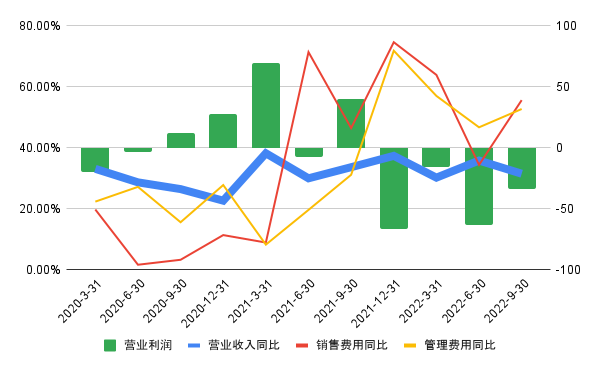
\includegraphics[width=0.8\linewidth]{img/rates.png}
    \end{center}
    \footnotesize{资料来源:Wind}
\end{figure}

